
\documentclass{article}
\usepackage{hyperref}
\usepackage{amsmath}
\usepackage{graphicx}
\usepackage{float}
\usepackage[demo]{graphicx}
\usepackage{subfig}
\title{Population Dynamics in One Dimensional Circular Graph, Based on Moran Process}
\date{}
\begin{document}
\maketitle
\section{Abstract}
Random walk is a widely used method in stochastic processes to simulate biological phenomena such as bacterial growth or viral spread. However, these patterns are not random, but depend on various environmental and genetic factors that affect the fitness and behavior of the species. In this project, we generate an algorithm based on the Moran model to show how these factors influence the fixation probability and fixation time of a mutant and resident under periodic environmental fluctuations. A simple random walk approach based on first passage time theory was used to compute the fixation probability and time of the species.\\
Our results have implications for understanding the evolutionary dynamics of populations in changing environments.

\section{Introduction}
In this project, I simulate a one dimensional circular graph that contains two random walkers. The distance between walkers shows the number of each species, mutant(A) and resident(B).\\
there are two resource levels, low-resource
(poor) sites and high-resource (rich) sites (two-color scheme). The difference between fitnesses in poor and rich site denotes level of fitness heterogeneity in the system. Fitness heterogeneity level is proportional to the standard deviation of the fitness and for type A (type B) and is denoted by $\sigma_A(\sigma_B)$ respectively.
In this simplified scheme we can write the fitness sets a, b as,
\begin{equation}
   a = r_A + \sigma _A * c
\end{equation}
\begin{equation}
    b = r_B + \sigma _B * c
\end{equation}
where $r_A (r_B)$ is the mean fitness of type A(type B) and $c = (c_1, c_2, · · · , c_N)$ is the resource function at every location. For two-concentration level scheme we assume $c_i = −1 (+1)$ for poor (rich) resource sites respectively. We assume equal number of poor and rich sites.\\
Animation for showing the general form of the model can be found under the \textbf{model directory}.
\section{Reproduction and dying}
Each step of our model starts with 1 mutant/resident and N-1 resident/mutant. In each step walkers goes to the right or left with bellow probabilities:\\
\begin{equation}
    P_{left_A} = \frac{r_M+\sigma_M * c[i]}{total fitness}
\end{equation}
\begin{equation}
    P_{right_A} = \frac{r_R+\sigma_R * c[i]}{total fitness}
\end{equation}
\begin{equation}
    P_{left_B} = \frac{r_M+\sigma_M * c[i]}{total fitness}
\end{equation}
\begin{equation}
    P_{right_B} = \frac{r_R+\sigma_R * c[i]}{total fitness}
\end{equation}
Where A and B represent our walkers and R and M represent resident and mutant respectively. 
\subsection{Algorithm}
\begin{enumerate}
    \item Randomly choose a location for walker A
    \item $location_B = location_A + 1$
    \item Define $number of mutant = |location_B -location_A|$
    \item In each time step, according to eq.3 - eq.6, one of movements are chosen.
    \item calculate $|location_B -location_A|$ again.
    \begin{enumerate}
        \item if number of mutant = 0, mutant become extinct.
        \item else loop (3) and (4).
    \end{enumerate}
\end{enumerate}
\newpage
\section{Results}
\subsection{Condition for selection of non-neutral mutants as fitness standard deviations, $\sigma_A$ and $\sigma_B$ vary.}
\begin{figure}[H]
    \centering
  {{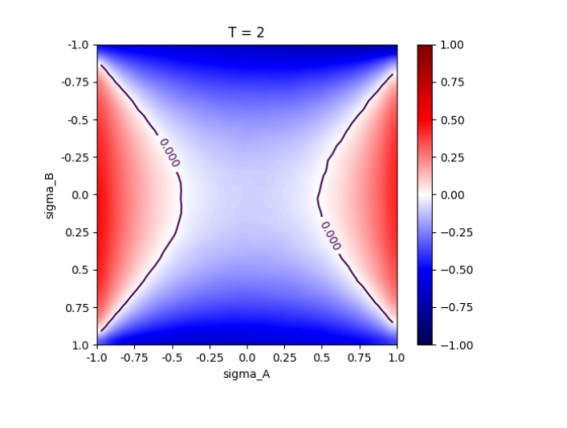
\includegraphics[width=5cm]{heat map.PNG}\\ }}%
    \qquad
  {{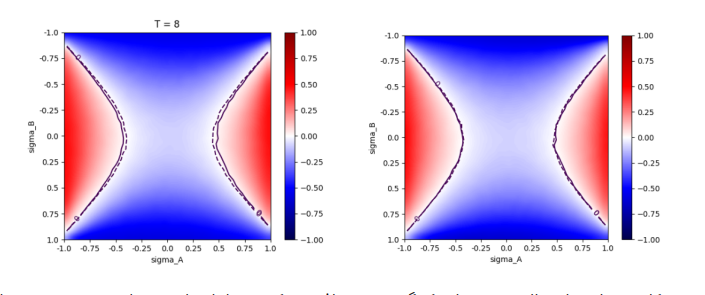
\includegraphics[width=10cm]{heat map 2.PNG} }}%
    \caption{The difference between the fixation probabilities, $\Delta\rho = \rho_A - \rho_B$ is plotted as $\sigma_A$ and $\sigma_B$ are varied for various periods T. T = 2, T = 4, and T = 8. The size of the graph is N = 16 and the inherent fitnesses are $r_A$ = 1.1, $r_B$ = 1. The dashed lines represent $\rho_A = \rho_B$ and the solid ones $\rho_A = \rho_B$ in a 2-chromatic cycle (T = 2).}%
\end{figure}
\subsection{Fixation probability of an advantageous mutant vs $\sigma$, and period, T.}
\begin{figure}[H]
    \centering
    \subfloat[\centering $\sigma_A = \sigma_B$]{{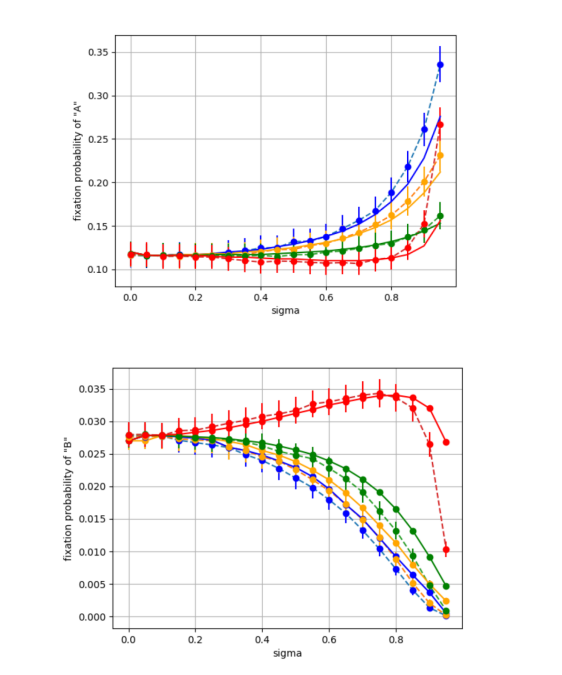
\includegraphics[width=5cm]{vertical move.PNG} }}%
    \qquad
    \subfloat[\centering $\sigma_A = - \sigma_B$]{{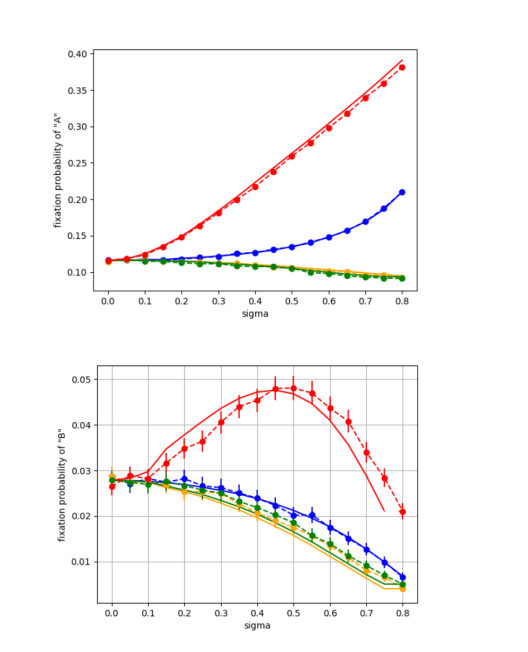
\includegraphics[width=5cm]{vertical move 2.PNG} }}%
    \caption{Fixation probability of an advantageous mutant (type A and B) plotted vs.$\sigma$ for different periods. The inherent fitnesses are $r_A$ = 1.1, $r_B$ = 1 and the fitness heterogeneity obeys the rule of Eq.1 and Eq.2. The dashed lines represent our model and the solid line represent analytical solution. Blue line represents T=2, yellow T=4, green T=8 and red T=16. }
\end{figure}
As the period is increased, time to fixation is increased much significantly along the $\sigma_A = - \sigma_B = \sigma$ axes which represents completely asymmetric interactions. In this scenario, both random walkers tend to go to the same direction whether left or right and reach to each other. Therefore, they meet each other After more time has passed in comparison with $\sigma_A =  \sigma_B = \sigma$ scenario. For example at $\sigma_A =  \sigma_B = 0.8$ in the largest period, we have the fixation time=$10^9$ while for a uniform environment, it is $10^3$. This is 6 order of magnitude increase in
time to fixation due to heterogeneity.
\subsection{Scaling of fixation time with N}
In a regular Moran process, one individual is randomly chosen to reproduce and another to die in each time step. It is possible that the same species is chosen for both actions, so the total number of each species does not change. In our model, each time step involves one of the walkers moving, which changes the total number of each species. Therefore, our model does not have time steps that the population does not change. This is like skipping some time steps that do not affect the overall shape of the population. Therefore, although the graphs for fixation time look similar to the analytical solution, the numbers are significantly lower, indicating that we can observe the density of our population with our model faster.\\
\begin{figure}[H]
    \centering
    \subfloat[\centering $T=2$, right graph represents $\sigma_A = \sigma_B$ and left one represents $\sigma_A = - \sigma_B$]{{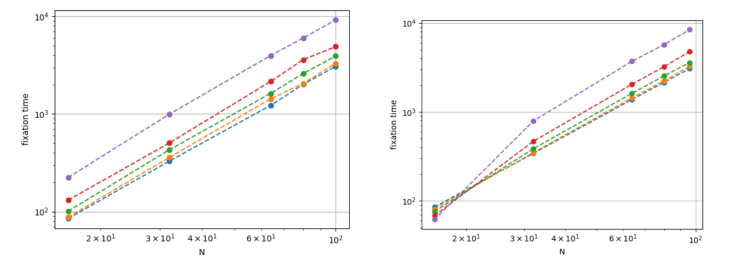
\includegraphics[width=10cm]{time.PNG}}}%
    \qquad
    \newline
    \subfloat[\centering $T=N$, $\sigma_A = \sigma_B$]{{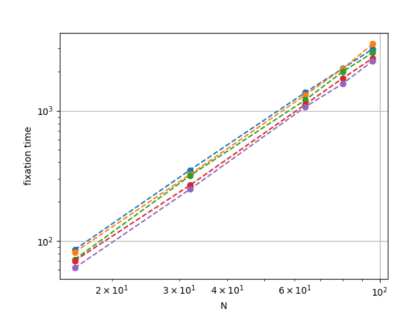
\includegraphics[width=5cm]{time 2.PNG} }}%
    \caption{Fixation time is plotted vs. N for the period T = 2, N in the case of $r_A = r_B = 1 $ and $\sigma_A = \sigma_B$ and $\sigma_A = - \sigma_B$ selected values of σ = 0, .2, .4, .6, .8. a) (log-log plot). For (a) we observe power-law scaling fixation time = $N^\alpha$ and for (b) we observe fixation time = $exp(\alpha N)$.}
\end{figure}
\subsection{Effect of fitness shift on the fixation probability}
How does changing the fitness distribution in the population affect the mutant type’s fitness?\\
We can explore this by using the same square-wave fitness functions as before, but with a phase difference between $a_i$ and $b_i$ as previously suggested. The fixation probability of types A and B depend on the phase difference relative to the symmetric interaction heterogeneity model. The difference becomes larger as the phase shift approaches $\frac{\pi}{2}$ and the heterogeneity amplitude $\sigma$ grows.
\vspace{-1cm}
\begin{figure}[H]
    \centering
    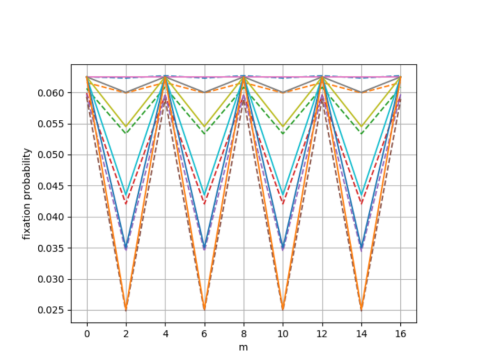
\includegraphics[width=0.5\linewidth]{shift.PNG}
    \caption{Fixation probability of an inherently neutral mutant is plotted vs. m in the periods T = 4 for
different values of $\sigma = [0, 0.2, 0.4, 0.8]$. A 16-node cyclic graph is considered and at m = 0, the rule of Eq.1 and Eq.2 are applied to the fitness pattern. The inherent fitnesses are considered to be $r_A = r_B = 1$.}
\end{figure}
\end{document}